\documentclass[twocolumn,10pt,a4j]{jsarticle}
\usepackage{kougai}
\usepackage{dcolumn}


\title{OffscreenCanvasを用いたシミュレータ教材の開発}
\author{1532040 岡本 悠祐  指導教員 須田 宇宙 准教授}
\date{}
 
\begin{document}
\maketitle
\section{はじめに}
シミュレータ教材は不可視現象を可視化する教材である.そのため,イメージが困難な事象への理解を促す手法として有用である.
e-Learningの普及に伴いシミュレータ教材の活躍の場が増加し,様々な分野に対応したシミュレータ教材と効率的な開発手法が必要とされている.

磁場や音場などの波形を可視化するシミュレータにおいてFTDT(Finite-difference time-domain )法が広く用いられているが演算回数が多いことから処理速度は決して速くない.
本研究室では昨年,FTDT法を用いたシミュレータ教材をGPUに適用しCPUとの処理速度を比較する研究が行われた.その結果,教材は大幅に処理速度が向上したが,ソースコードの変更箇所が多く,
複雑なため容易に実装できないという問題点が浮上した.

%この問題点はJavaScriptでWebWorkerを活用し,描画を行うOffscreenCanvasを利用することで緩和されると考える.

本研究ではOffscreenCanvasを利用したFTDT法を用いたシミュレータ教材の開発を行い,ソフトウェアの生産性と処理速度を昨年開発されたシミュレータ教材と比較することで,有用性の検証を行うことを目的とする.

\begin{comment}

\section{WebWorkerとOffscreenCanvas}
\subsection{WebWorker}
WebWorkerはJavaScriptでマルチスレッド処理を可能にするAPIである.Workerを利用するには処理ごとにファイルを分ける.
また,Worker上で描画を行うことができないため描画処理を行いたい場合は,Workerを定義するメインのスレッドに対して描画処理を渡す必要がある.

\subsection{OffscreenCanvas}
OffscreenCanvasはWebWorkerを利用してWorker上で描画処理を可能にするAPIである.

事前にCanvasタグをHTMLないしJavaScriptで生成し,Workerに処理を譲渡,描画まで行うため,Workerより必要な処理が少なく手軽に実装できる.

\end{comment}

\section{開発したシミュレータ教材}
本研究ではOffscreenCanvasを利用したシミュレータ教材の有用性の検証を行う.プログラムは昨年度本学の卒業論文である「GPU利用によるシミュレータ教材の演算速度」を拡張し,処理速度とソースコードの比較を行う.

図\ref{fig:one}は複数の音源から発生する音場を可視化したシミュレータである.キャンバスを左右に分けることにより,負荷を分散させた.


\begin{figure}[htbp]
  \begin{center}
   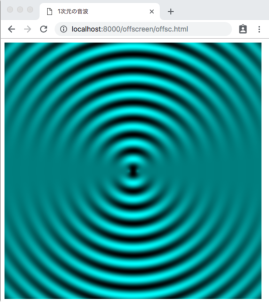
\includegraphics[width=30mm]{sim.pdf}
  \end{center}
  \caption{開発したシミュレータ}
  \label{fig:one}
\end{figure}

\section{検証方法}
昨年のシミュレータの処理にかかる時間や,プログラムが変更した箇所の比較を行う.
 
1,000回計算する際の時間を計測し,10,000回まで行った.
比較に昨年度に制作されたプログラム2つ,昨年度の論文で演算速度の比較を行ったCPUとGPU向けのプログラムと本論文で開発したOffscreenCanvas,WebWorkerを利用した4つのシステム用いた.
本梗概では,昨年度制作されたプログラムのうち,CPUを対象としたプログラムをCPUとし,GPU向けのプログラムをGPUと称する.


計測に使用した機材のスペックを表 \ref{tab:tab1}に示す.

\begin{table} [h]
\centering
\caption{使用した機材のスペック}
	\begin{tabular} {| c | c |} \hline
	OS & macOS High Sierra \\ \hline
	メモリ & 32GB \\ \hline
	CPU & 3.2GHz Intel Core i5(コア数4) \\ \hline
	GPU & NVIDIA GeForce GT 775M 1024MB\\ \hline
	\end{tabular} 
	\label{tab:tab1}
\end{table}



\section{検証結果}
CPUを基準とした各システムの処理に費やした時間を式(\ref{eq:eq1})に当てはめて求めた.

キャンバスを分割したWebWorkerとOffscreenCanvasは処理時間が遅い方を参照する.その結果を表\ref{tab:tab2}に記した.

その結果,WebWorkerが一番速く処理を行えることがわかった.
\begin{equation}
 処理時間比率 = \frac { 各手法10,000回の処理時間 \, \mathrm{(ms)}} { 基準10,000回の処理時間\, \mathrm{(ms)} } 
\label{eq:eq1}
\end{equation}


\begin{table} [h]
\centering
\caption{各種法の処理速度比較}
	\begin{tabular} {| c | l |} \hline
	利用したシステム & 処理時間比率 \\ \hline
	GPU & 0.810988 \\ \hline
	OffscreenCanvas & 0.80789763 \\ \hline
	WebWorker & 0.795556697 \\ \hline
	\end{tabular} 
	\label{tab:tab2}
\end{table}
シミュレータのアルゴリズムを変更することはなかった.また,図\ref{fig:two}のようにOffscreenCanvasはworkerを宣言するメインの処理がWebWorkerと比較して少なくなることがわかった.
\begin{figure}[htbp]
  \begin{center}
   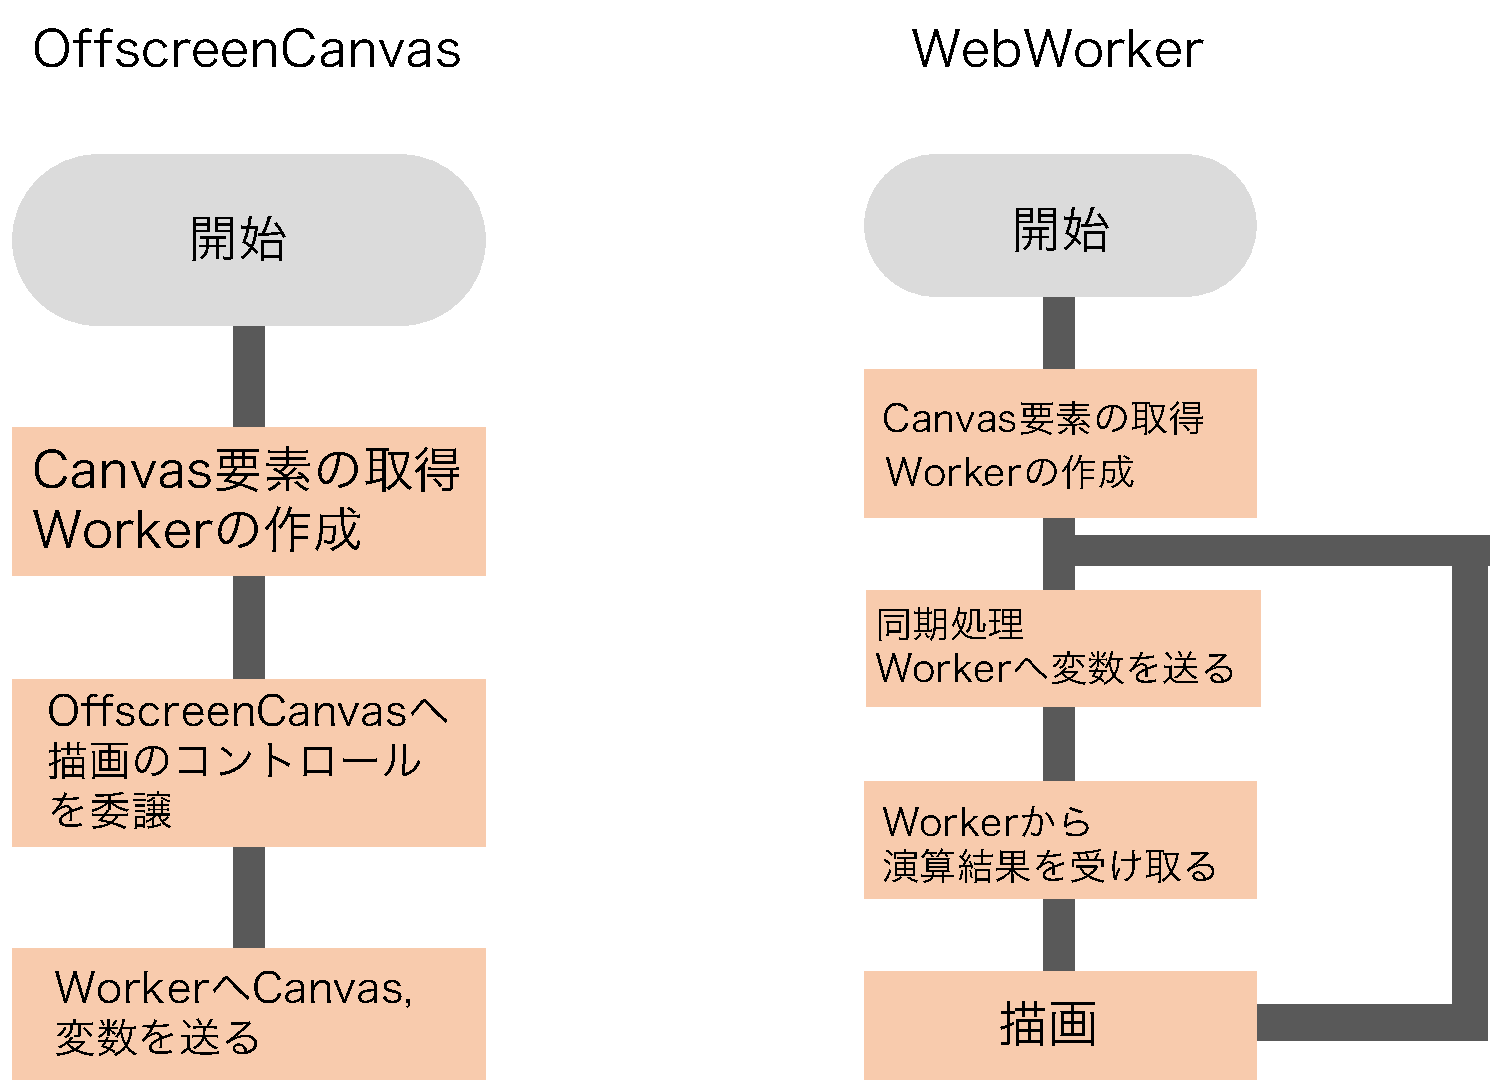
\includegraphics[width=60mm]{chart.pdf}
  \end{center}
  \caption{メインの処理}
  \label{fig:two}
\end{figure}
%Workerのみと違いworkerを宣言するメインではデータのデータの引き渡しがないだけでなく,左右のキャンバスを整合性をとる必要がないことからOffscreenCanvasはWorkerより実装が容易である.

\section{終わりに}
本研究ではOffscreenCanvasのFTDT法を用いたシミュレータへの有用性を検証した.
OffscreenCanvasは処理速度向上に役立ち,WebWorkerより実装がしやすいことがわかった.
今回WebWorkerの処理が一番早かったのは
\begin{thebibliography}{99}

	\bibitem{book}中嶋 大貴:``GPU利用によるシミュレータ教材の演算速度'',本学卒業研究,(2018)
\end{thebibliography}
\end{document}
